\section{Auswertung}
\label{sec:Auswertung}

\subsection{Überprüfung der Stabilität}
\label{subsec:stabilitaet}
Die Messwerte für den realisierten Laser mit einem flachen und einem sphärischen
Spiegel befinden sich in Tabelle \ref{tab:plankonkav}. In Abbildung \ref{fig:plankonkav}
sind die gemessenen Stromstärken $I$ gegen die Resonatorlängen $L$ aufgetragen.
Zudem wird eine lineare Ausgleichrechung der Form
\begin{equation*}
  f(L)=a L+b
\end{equation*}
durchgeführt. Für die Berechnungen wird Python 3.7.1, unterstützt von dem Paket
NumPy \cite{numpy} genutzt. Für die Grafiken
wird die Python Bibliothek matblotlib \cite{matplotlib} verwendet.
Die Ausgleichsrechnungen werden mithilfe von SciPy \cite{scipy} durchgeführt.
Für die Parameter $a$ und $b$ ergeben sich die Werte
\begin{align*}
  a&= \SI{2.61(029)}{\micro\ampere\per\centi\per\metre}\,,\\
  b&= \SI{214(18)}{\micro\ampere}\,.
\end{align*}

\begin{figure}
  \centering
  \includegraphics{build/plankonkav.pdf}
  \caption{Darstellung der Messwerte sowie der Ausgleichsfunktion für den
  Resonator aus einem flachen und einem sphärischen Spiegel.}
  \label{fig:plankonkav}
\end{figure}

Die Messwerte für den Resonator aus zwei sphärischen Spiegeln befinden sich in
Tabelle \ref{tab:konkavkonkav}. In Abbildung \ref{fig:konkavkonkav} sind die gemessenen Stromstärken gegen die Resonatorlänge aufgetragen. Außerdem wird eine
Ausgleichsfunktion der Form
\begin{equation*}
  f(L)=a L^2 + b L + c
\end{equation*}
angesetzt. Es ergeben sich die Parameter
\begin{align*}
  a&= \SI{0.097(017)}{\micro\ampere\per\centi\per\metre\squared}\,, \\
  b&= \SI{-21(4)}{\micro\ampere\per\centi\per\metre}\,, \\
  c&= \SI{1.15(020)e3}{\micro\ampere}\,.
\end{align*}

\begin{figure}
  \centering
  \includegraphics{build/konkavkonkav.pdf}
  \caption{Darstellung der Messwerte sowie der Ausgleichsfunktion für den
  Resonator aus zwei sphärischen Spiegeln.}
  \label{fig:konkavkonkav}
\end{figure}

\subsection{Vermessung der Moden}
\label{subsec:moden}

Die gemessenen Werte für die TEM$_{\mathrm{00}}$ Mode befinden sich in den Tabellen \ref{tab:tem00a} und \ref{tab:tem00b}. In Abbildung \ref{fig:tem00} sind sie
grafisch dargestellt. Die Werte zeigen nicht den theoretisch zu erwartenden gaußförmigen
Verlauf. In Abbildung \ref{fig:bild} ist ein Bild dieser Mode eingefügt. Auch dort
ist im Zentrum eine geringere Intensität zu erkennen.

Trotz der Abweichungen wird eine Ausgleichsrechnung mit einer gaußförmigen Funktion
\begin{equation*}
  I_{0,0}(L)=I_{\text{max}} \exp\left(-2 \left(\frac{L-d}{\omega}\right)^2\right)
\end{equation*}
durchgeführt. Dabei ist $I_{\text{max}}$ der maximale Strom, $d$ eine Verschiebung in
x-Richtung und $\omega$ der Strahlradius. Es ergeben sich die Parameter
\begin{align*}
  I_{\text{max}}&=\SI{597(29)}{\micro\ampere} \,,\\
  d&= \SI{-3.2(8)}{\milli\metre} \,, \\
  \omega&=\SI{27.8(17)}{\milli\metre} \,.
\end{align*}

\begin{figure}
  \centering
  \includegraphics{build/tem00.pdf}
  \caption{Darstellung der Messwerte sowie der Ausgleichsfunktion für die TEM$_{\mathrm{00}}$ Mode.}
  \label{fig:tem00}
\end{figure}

\begin{figure}
  \centering
  \includegraphics[width=0.7\textwidth]{data/tem00.png}
  \caption{Bild der TEM$_{\mathrm{00}}$ Mode. Deutlich zu erkennen ist eine schwächere Intensität im Zentrum.}
  \label{fig:bild}
\end{figure}


Die Messwerte für die TEM$_{\mathrm{01}}$ Mode sind in den Tabellen \ref{tab:tem01a} und \ref{tab:tem01b} aufgeführt. In Abbildung \ref{fig:tem01} sind sie grafisch dargestellt. Als Ausgleichsfunktion wird ein Produkt von Parabel und Gaußverteilung in der Form
\begin{equation*}
  I_{0,1}=I_{\text{max}}\left(\frac{L-d}{\omega}\right)^2 \exp\left(-2\left(\frac{L-d}{\omega}\right)^2\right)
\end{equation*}
angesetzt.
Die Ausgleichsrechnung liefert die Parameter
\begin{align*}
  I_{\text{max}}&=\SI{1.27(05)e3}{\nano\ampere} \,,\\
  d&=\SI{0.38(28)}{\milli\metre} \,,\\
  w&=\SI{15.0(4)}{\milli\metre} \,.
\end{align*}

\begin{figure}
  \centering
  \includegraphics{build/tem01.pdf}
  \caption{Darstellung der Messwerte sowie der Ausgleichsfunktion für die TEM$_{\mathrm{01}}$ Mode.}
  \label{fig:tem01}
\end{figure}

\subsection{Messung der Polarisierung}
\label{subsec:polarisierung}

In Tabelle \ref{tab:polarisation} befinden sich die Messwerte zur Intensität des
Laserstrahls in Abhängigkeit von dem Winkel des Polarisationsfilters. Diese Werte
sind in Abbildung \ref{fig:polarisation} graphisch dargestellt. Die Ausgleichsfunktion ist
\begin{equation*}
  f(\phi)=I_{\text{max}} \cos^2(\phi+\delta)\,.
\end{equation*}
Dabei ist $\phi$ der Winkel des Polarisationsfilters, $I_{\text{max}}$ ist der
maximale Strom und $\delta$ ist die Phasenverschiebung.
Die Ausgleichsrechnung liefert die Parameter
\begin{align*}
  I_{\text{max}}&=\SI{56.02(118)}{\micro\ampere} \,, \\
  \delta&=\SI{19.32(105)}{\degree} \,.
\end{align*}

\begin{figure}
  \centering
  \includegraphics{build/polarisation.pdf}
  \caption{Darstellung der Messwerte sowie der Ausgleichsfunktion für die Intensität in
  Abhängigkeit vom Winkel des Polarisationsfilters.}
  \label{fig:polarisation}
\end{figure}

\subsection{Bestimmung der Wellenlänge}
\label{subsec:wellenlaenge}
Zur Bestimmung der Wellenlänge des Lasers wurden die Werte
\begin{align*}
  d_1&=\SI{6.3(2)}{\centi\metre} \,,\\
  d_2&=\SI{6.2(2)}{\centi\metre}  \,,\\
  l&=\SI{95.7(2)}{\centi\metre} \,.
\end{align*}
gemessen.
Die beiden Messwerte für $d$ werden gemittelt und es ergibt sich $\SI{6.25(14)}{\centi\metre}$
\footnote{Ist $f$ eine Funktion, die von unsicheren Variablen $x_i$ mit
Standardabweichungen $\sigma_i$ abhängt, so ist die Unsicherheit von f gegeben durch
  $\sigma_f = \sqrt{
    \sum\limits_{i = 1}^N
      \left( \frac{\partial f}{\partial x_i} \sigma_i \right)^{\!\! 2}
  }\,.$
}
, wobei die Unsicherheit sich zu $\sigma_d = \frac{1}{2} \sqrt{\sigma_{d_1}^2+\sigma_{d_2}^2} = \frac{\sqrt{2}}{10}\,\text{cm}$
bestimmt.
Mithilfe des Zusammenhangs
\begin{equation*}
  \lambda= g \sin \left(\arctan\left(\frac{d}{l}\right)\right)
\end{equation*}
lässt sich daraus die Wellenlänge berechnen. Dabei ist $l$ der Abstand zwischen
Gitter und Schirm, $d$ der Abstand der ersten Hauptmaxima vom nullten Hauptmaximum
auf dem Schirm und g ist die Spaltbreite des Gitters. Das verwendete Gitter hat eine
Spaltbreite von $10^{-5}$\,m. Damit ergibt sich für die Wellenlänge des Lasers der Wert
\begin{align*}
  \lambda=\SI{652(15)}{\nano\metre}\,.
\end{align*}
Die Unsicherheit von $\lambda$ lässt sich mit
\begin{equation}
  \sigma_\lambda = \sqrt{\frac{d^{2} g^{2} \sigma_{l}^{2}}{l^{4} \left(\frac{d^{2}}{l^{2}} + 1\right)^{2}} + \frac{g^{2} \sigma_{d}^{2}}{l^{2} \left(\frac{d^{2}}{l^{2}} + 1\right)^{2}} {\left (\frac{d}{l} \right )}}
\end{equation}
berechnen.
Der theoretisch zu erwartende Wert ist $\lambda= 632,8$\,mm. Der experimentell bestimmte
Wert weicht davon um $3,0$\,\% ab.
